\section{XPP: Rovers}
\label{xpp-rovers}


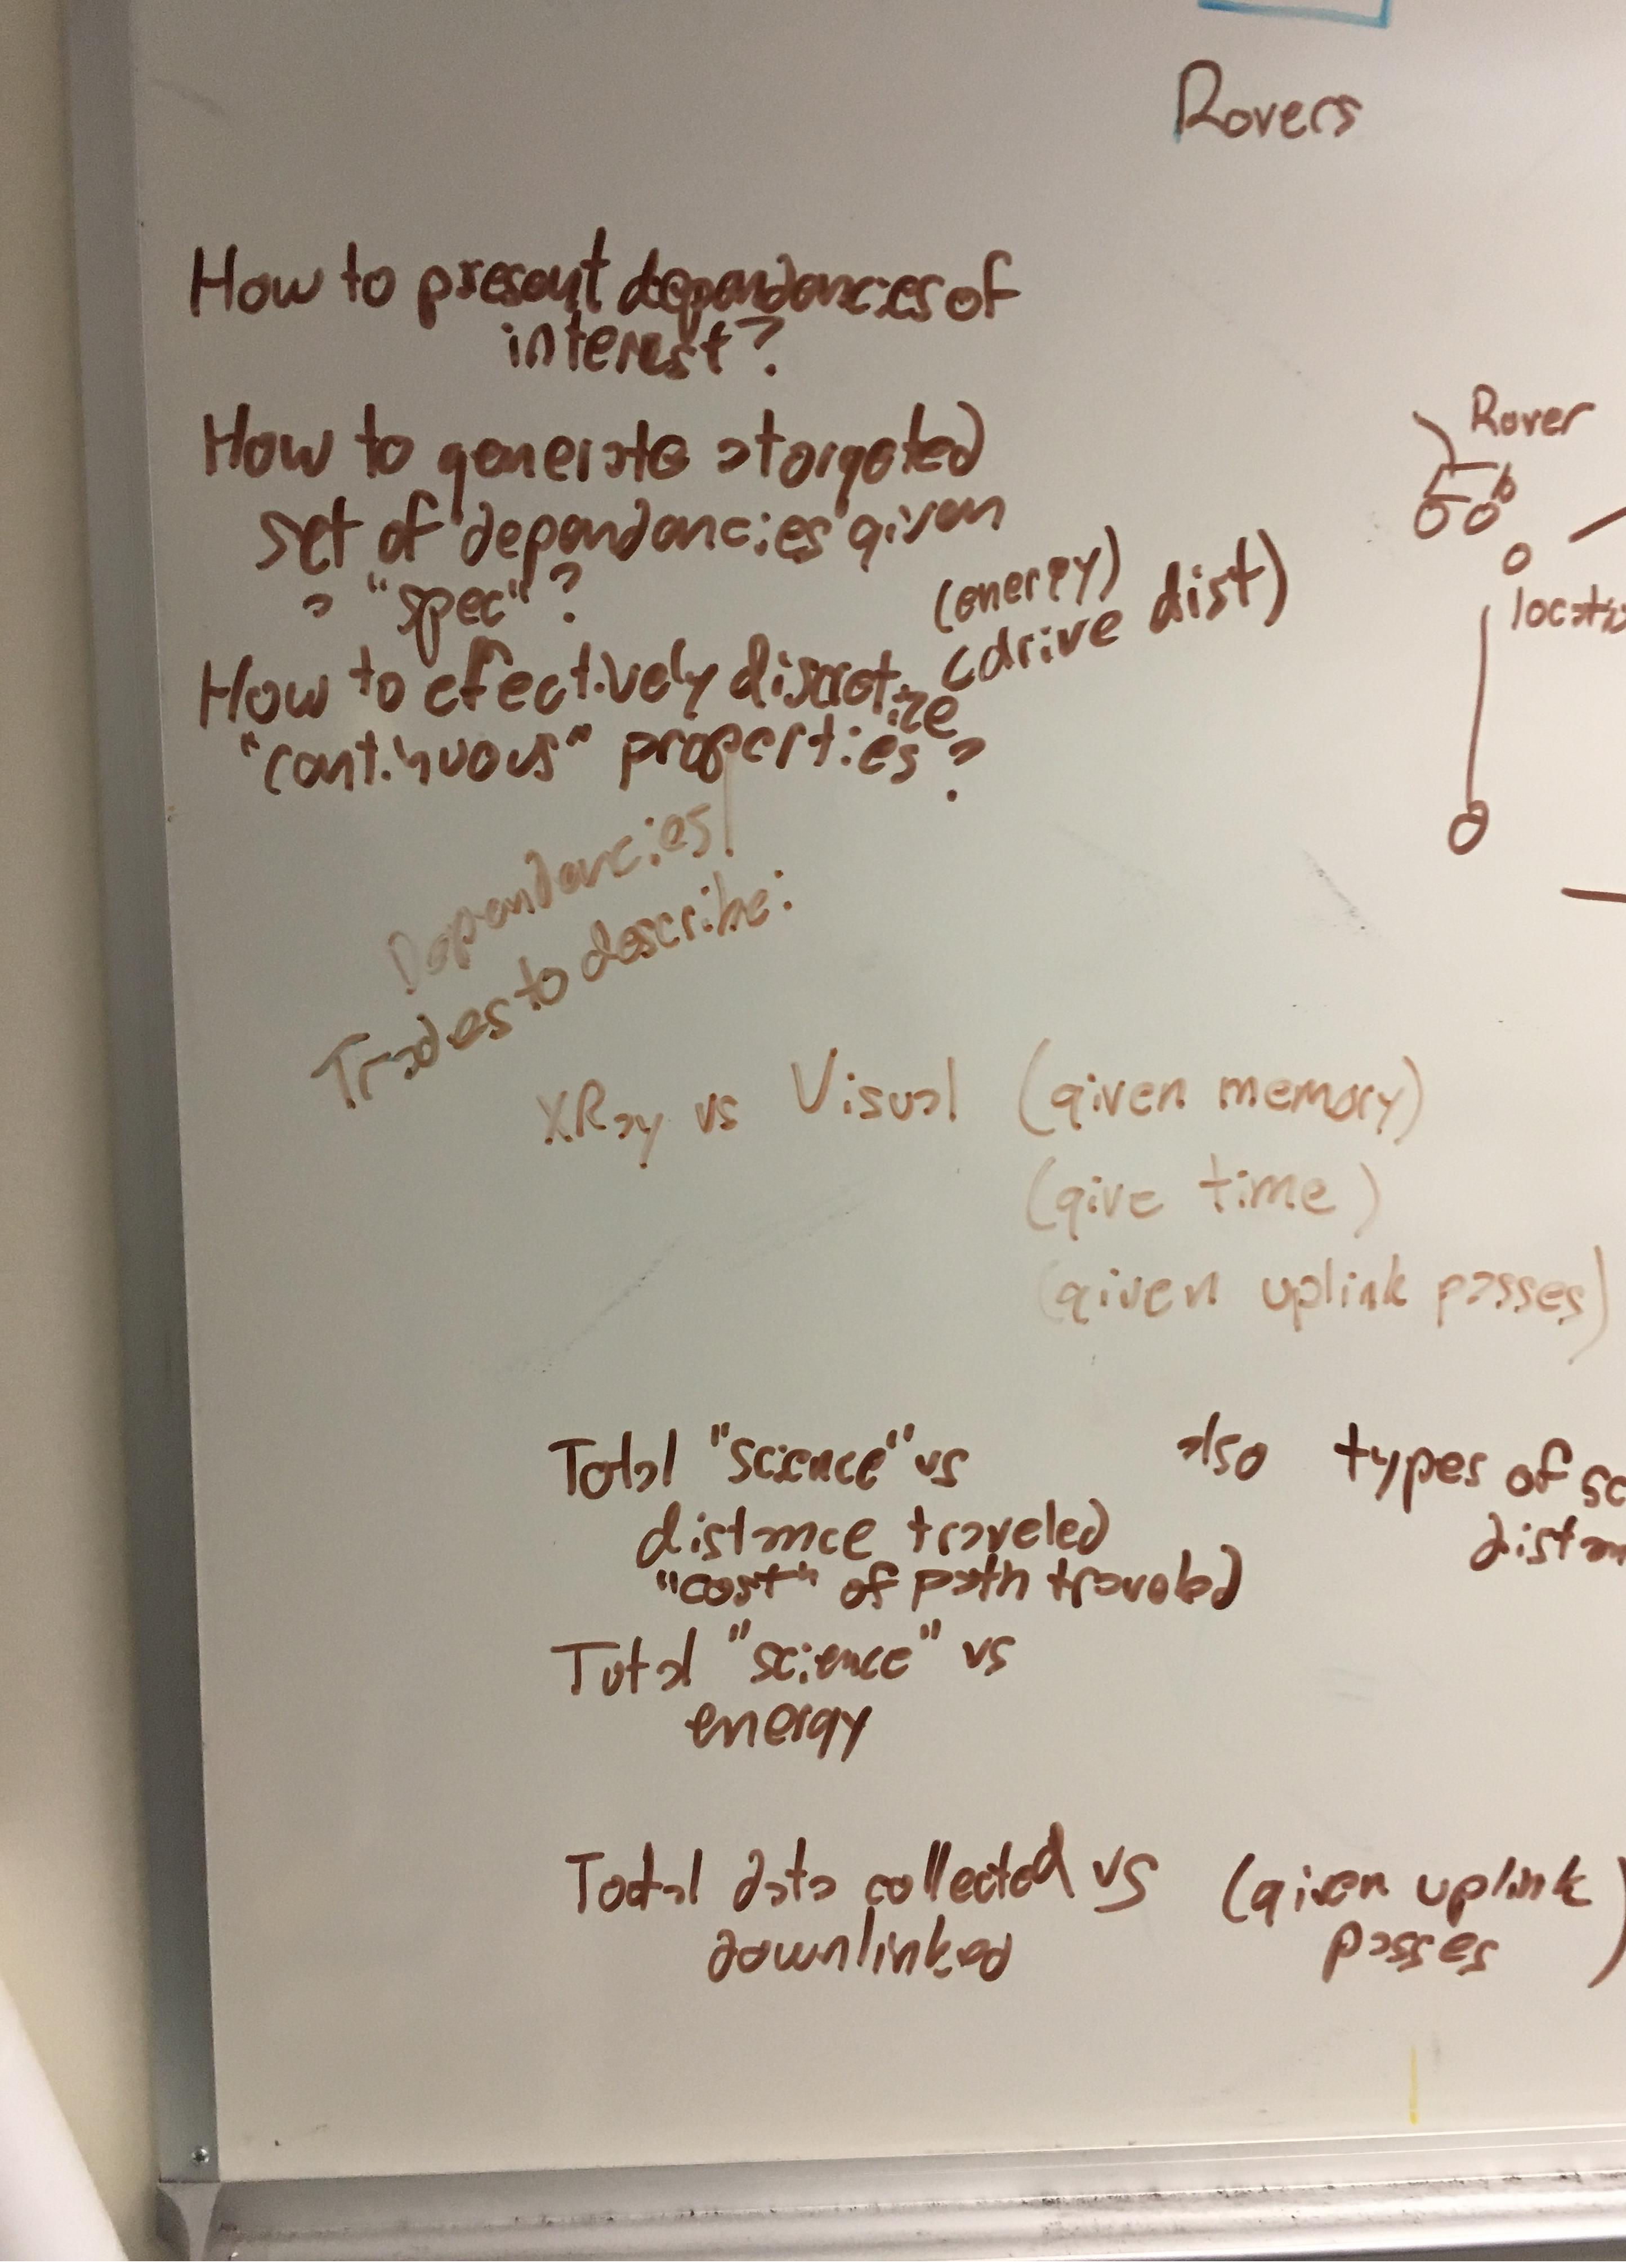
\includegraphics[height=8.0cm]{IMAGES/jeremy-whiteboard-rovers-1.JPG}
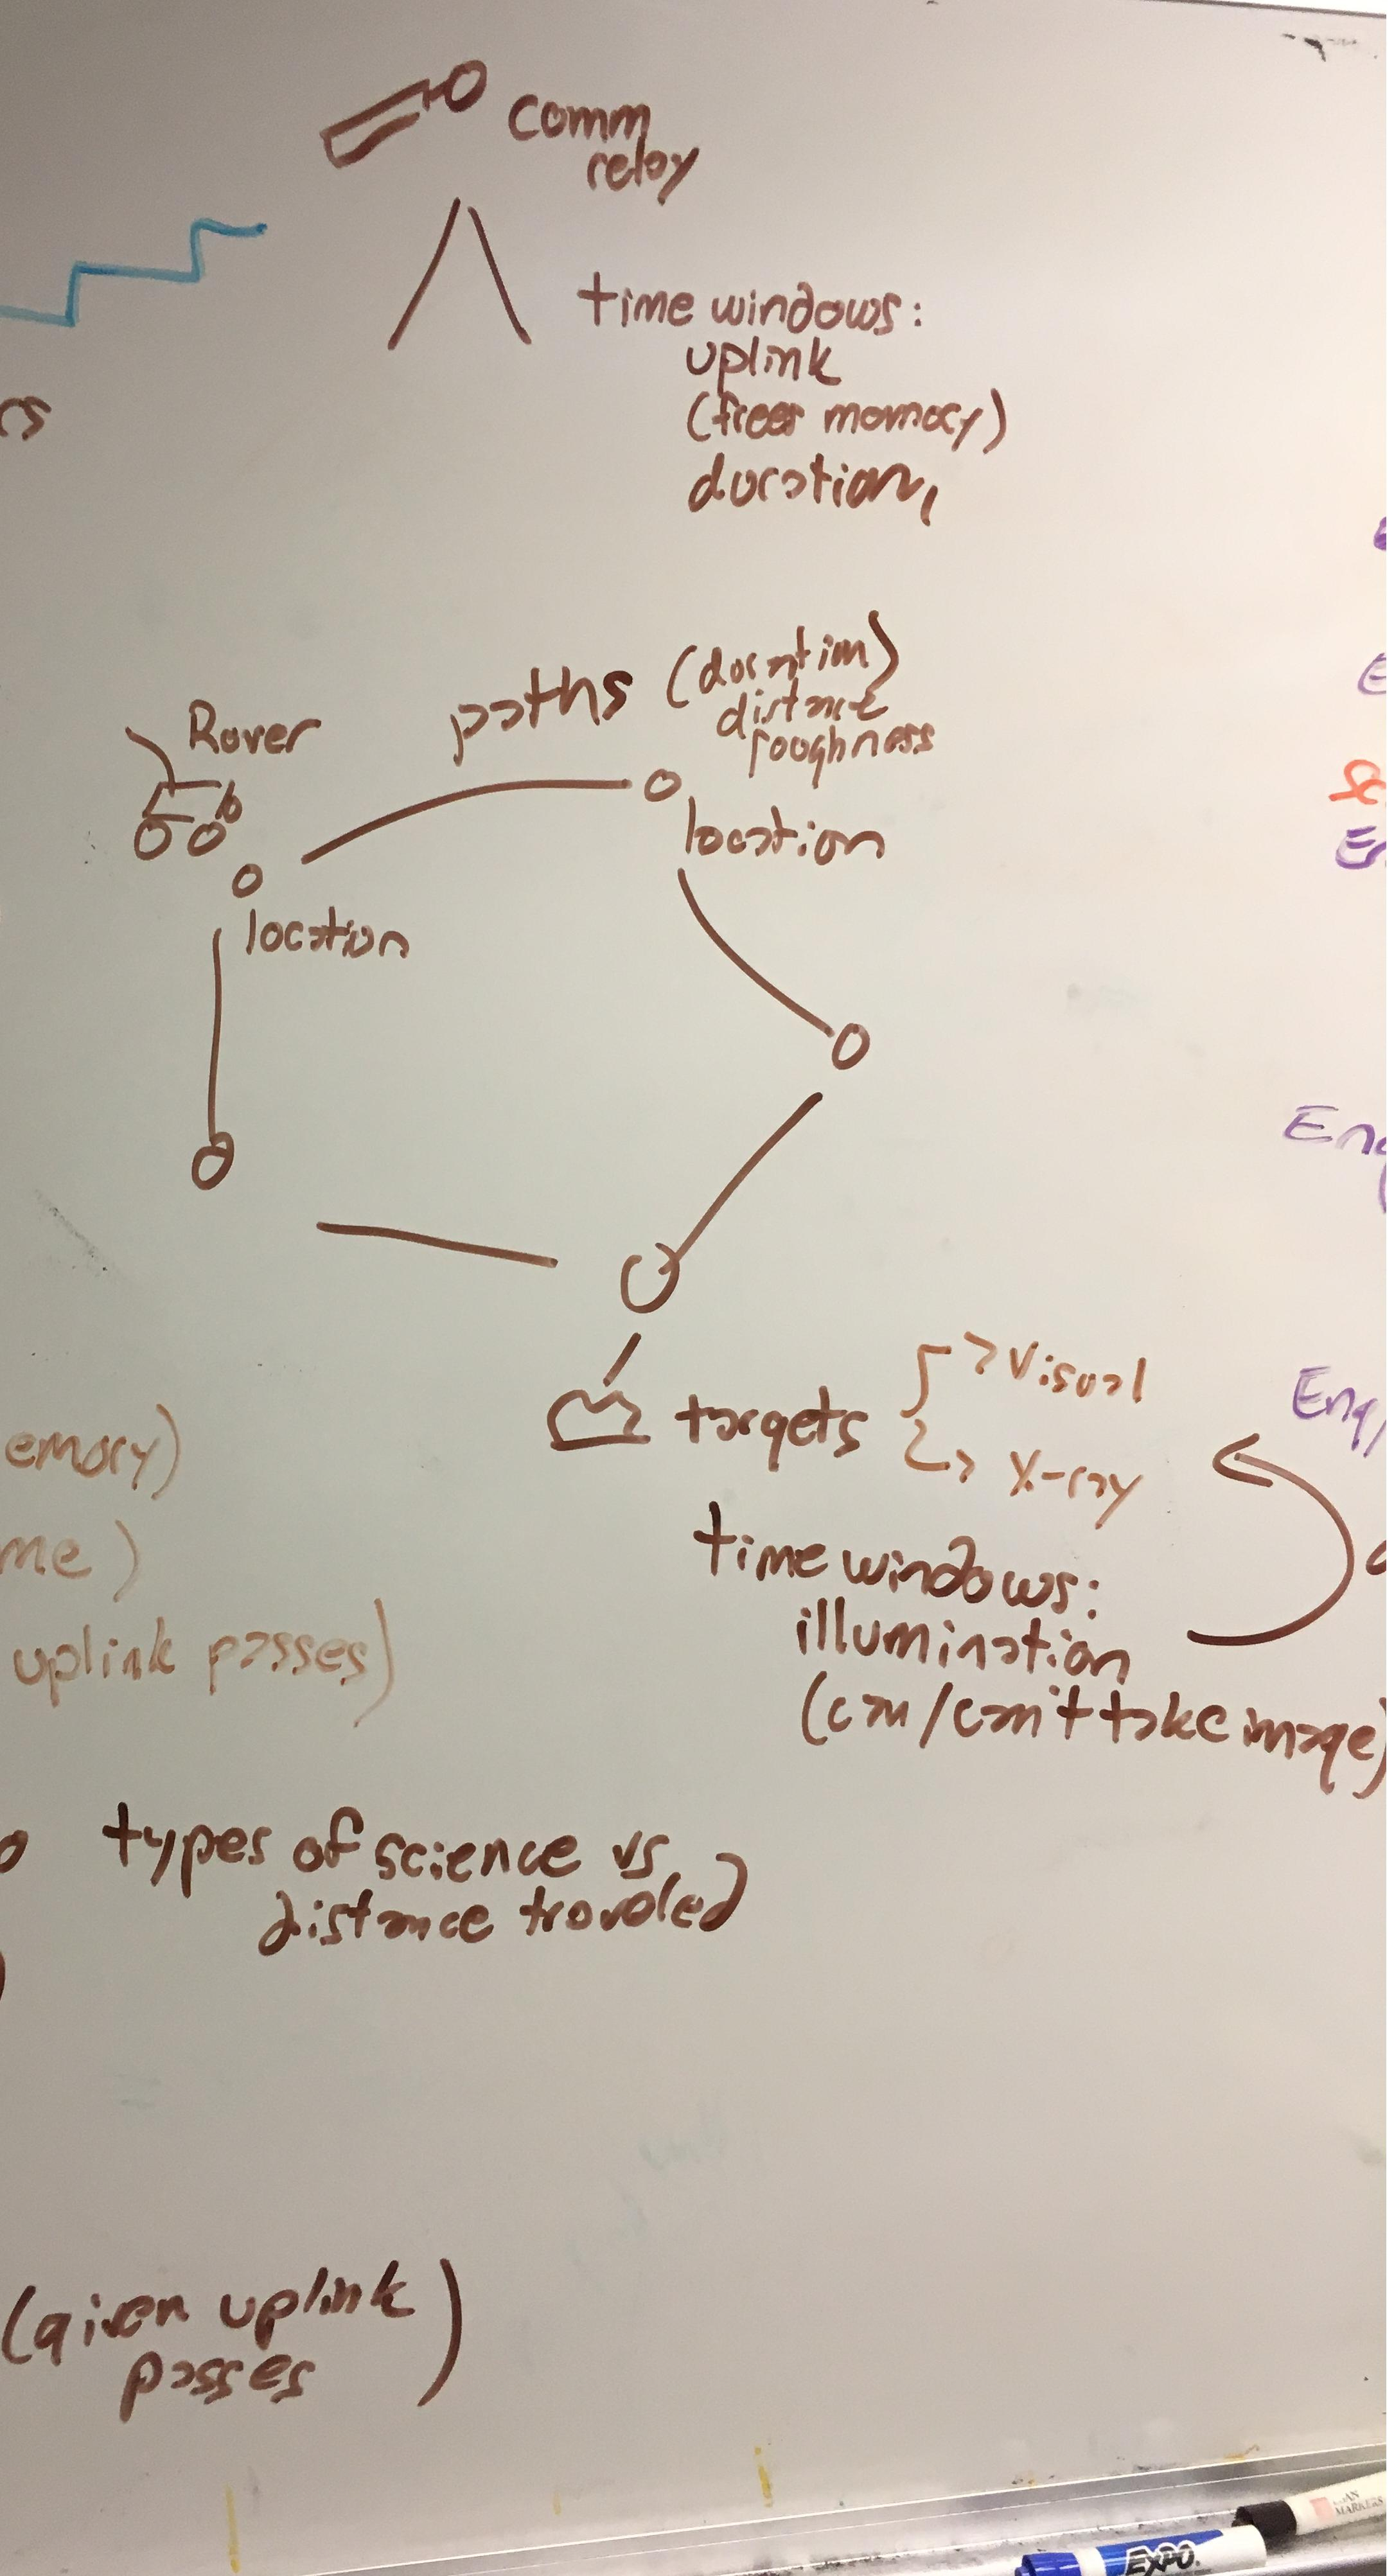
\includegraphics[height=8.0cm]{IMAGES/jeremy-whiteboard-rovers-2.JPG}
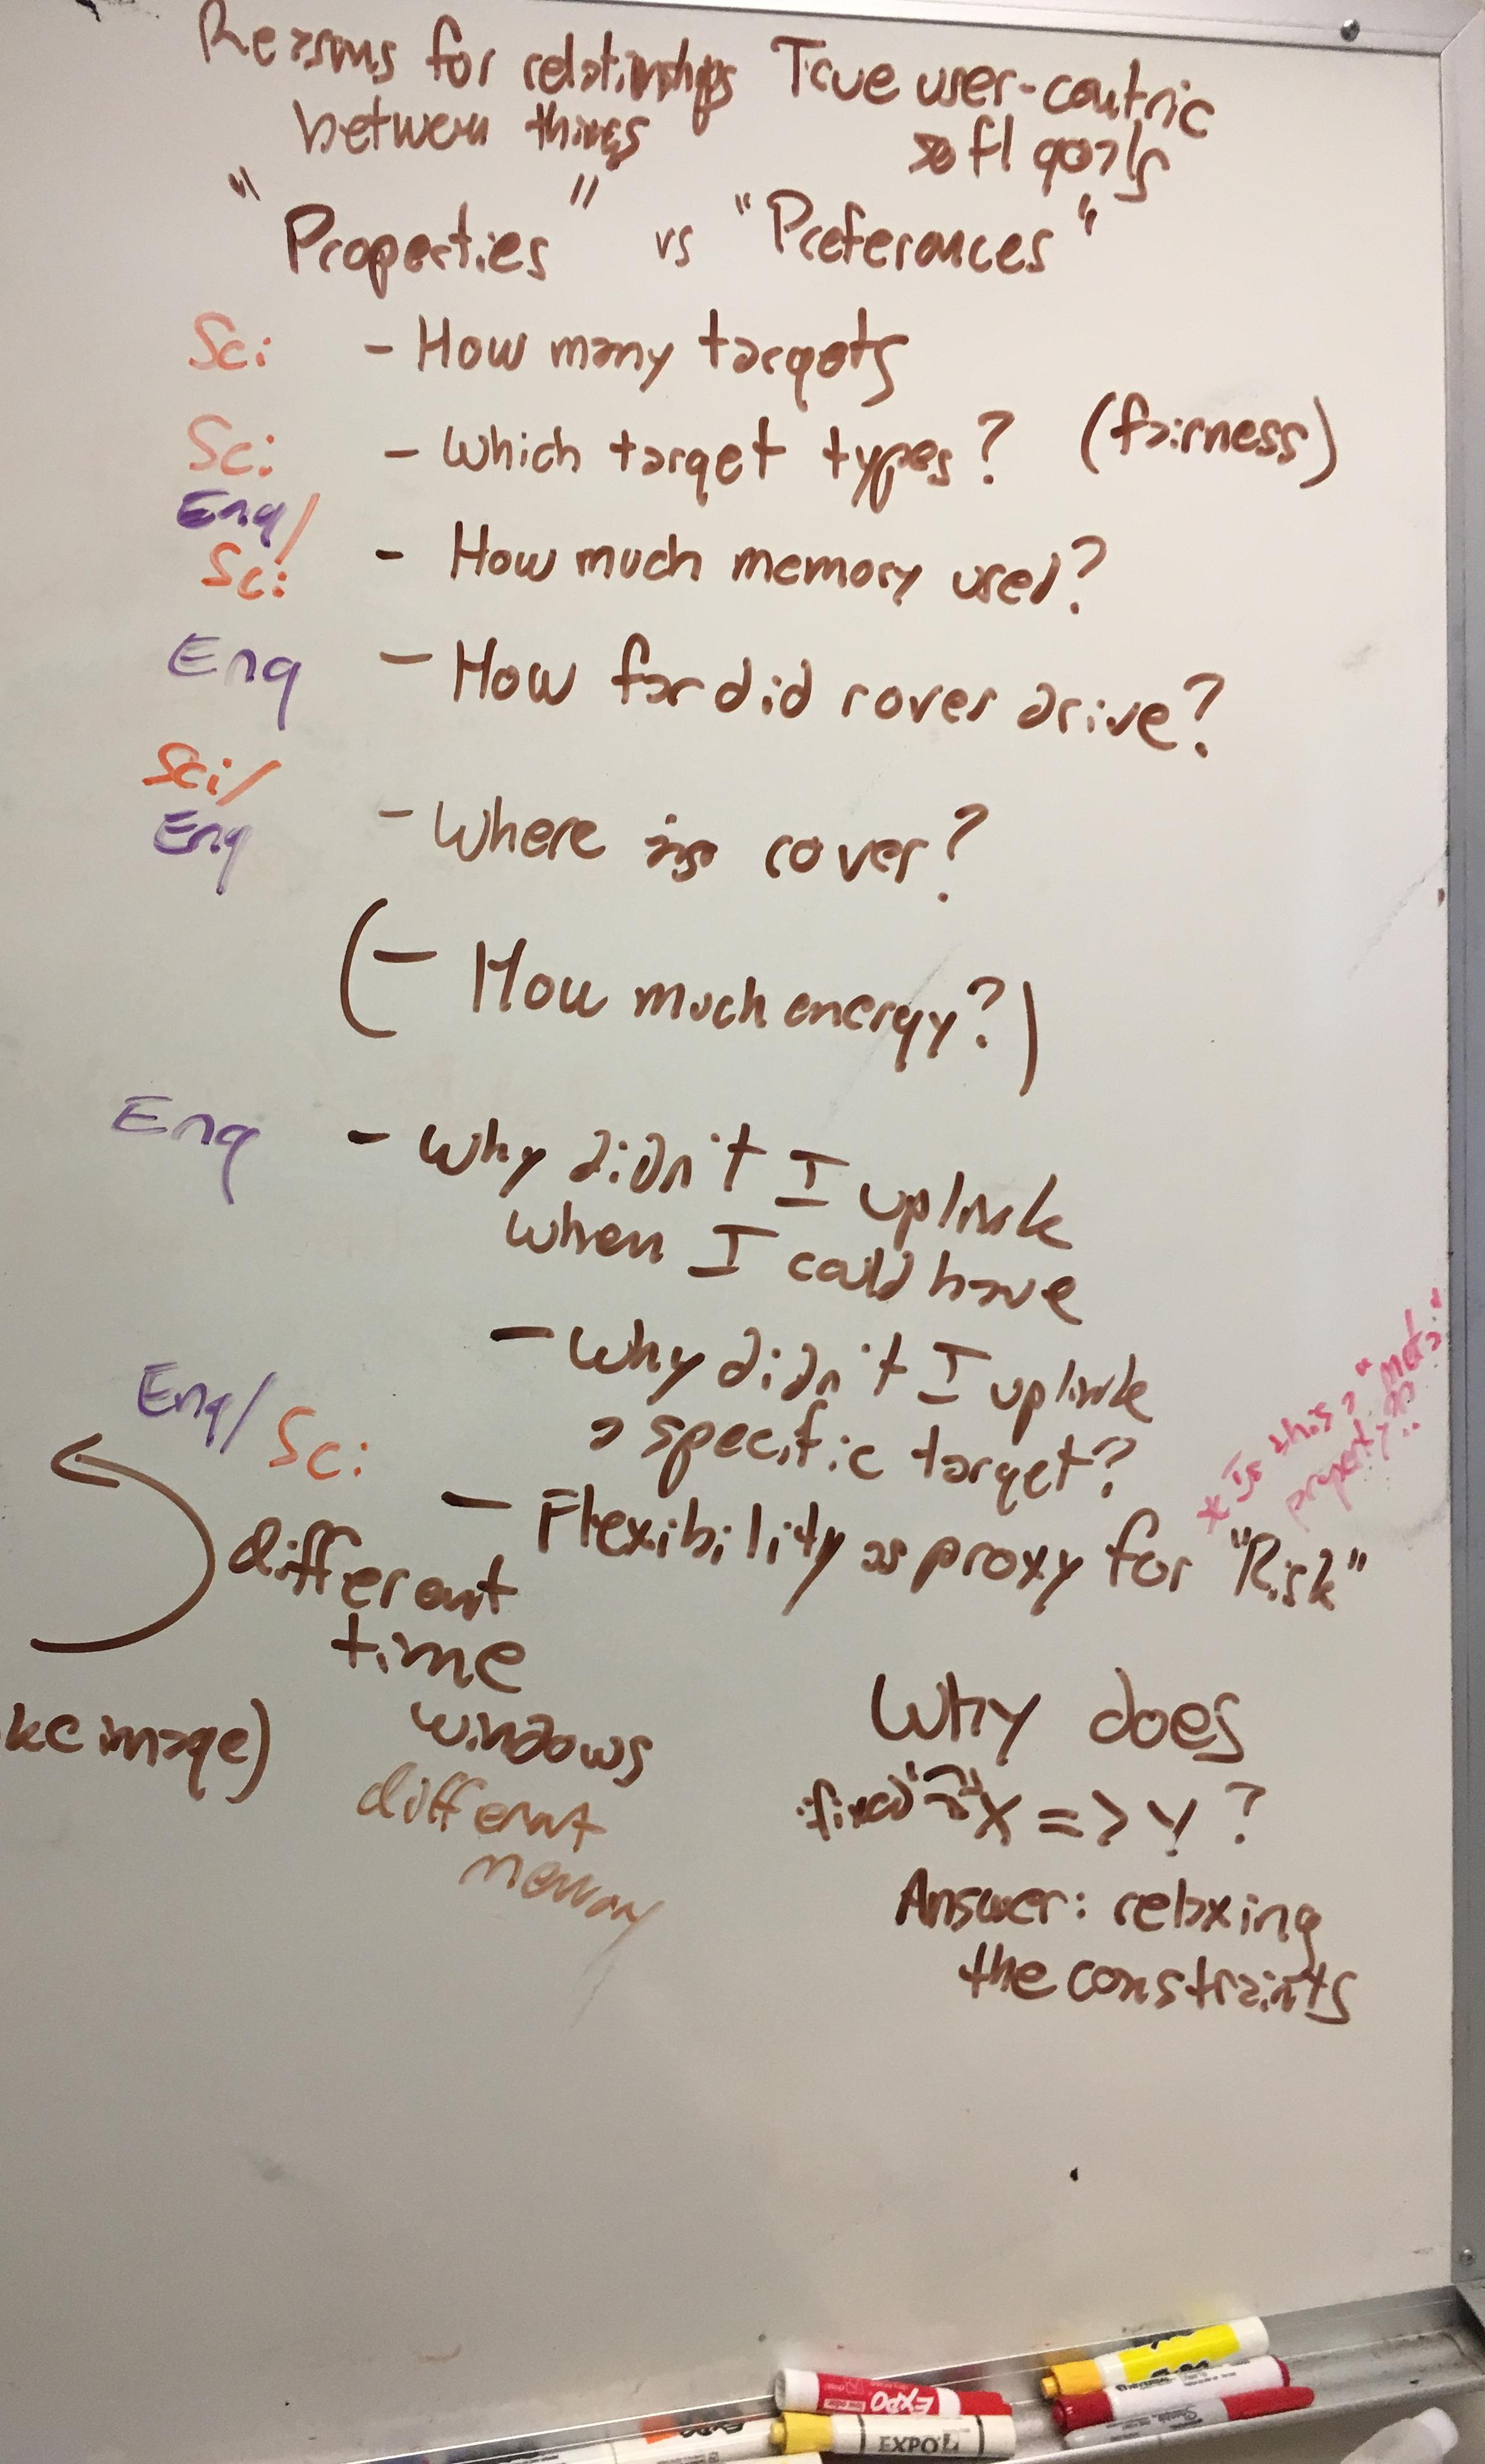
\includegraphics[height=8.0cm]{IMAGES/jeremy-whiteboard-rovers-3.JPG}


\subsection{Rovers model and properties}
\label{xpp-rovers:model}

Model: 
\begin{itemize}
\item rover
\item waypoints
\item paths: duration, cost for distance+roughness
\item targets: collection duration
\item target types (visual, x-ray, rock sample...)
\item feasability time windows for each target
\item amount of memory slots available (each target occupies one slot)
\item time windows for uplinking a given number of memory slots
\item energy level
\end{itemize}

Properties are grouped into ``dimensions'' meaningful to user, eg
different Boolean properties all discretizing amount of x-ray science
objectives achieved.


Property dimensions (that our objective is a function of):
\begin{itemize}
\item (scientists) fraction of targets collected by time point $T \geq
  X$?
\item (scientists) fraction of targets of type TT collected by time
  point $T \geq X$?
\item (scientists) distribution of fractions across types is fair?
\item (engineers) driving cost incurred by rover $\geq X$?
\item flexibility: slack in plan $\geq X$? 

  Serves as proxy for risk.

  (Or: how many concrete schedules does a given schedule permit?)
\item idle time in plan $\geq X$?

  When goals can't be achieved outside of specific time windows, idle
  time is often a consideration.  In cases like the rover domain where
  other 'non-goal-achieving' activities must be done (driving,
  uplinking), it may be hard to understand whether a plan looks good
  or bad from the perspective of idle-time. Intuitively, more science
  should translate to less idle time, but not always.  Furthermore,
  risk and idle time may be traded in interesting ways.

\end{itemize}


Property dimensions (that have causal influence on the above):
\begin{itemize}
\item \#memory slots available $\geq X$? [task property, not actionable]
\item maximal driving cost $\geq X$? [task property, actionable]
\item fraction of memory used at time point $T = X$?
\item rover at waypoint $X$?
\item target $X$ collected in time window $Y$?
\item uplink done in time window $Y$?
\item uplink done for target $X$ in time window $Y$?
\item amount of energy used $\geq X$?
\item amount of energy available $\geq X$? [model property! might be
  actionable]
\end{itemize}







\subsection{Rovers: expected dependencies and WHY/HOW questions}
\label{xpp-rovers:whyhow}


Example dependencies:
\begin{itemize}
\item A) fraction of targets of type x-ray collected at end of plan
  $\geq 40$\% $\Rightarrow$ fraction of targets of type visual
  collected at end of plan $< 20$\%.
\item B) \#memory slots available $< 7$ $\Rightarrow$ distribution of
  fractions across types is not fair.
\item C) uplink science objective A at time X $\Rightarrow$ don't
  achieve science objective B.
\end{itemize}

HOW questions: 
\begin{itemize}
\item eg A) how could this be improved? 

  \#memory slots available $\geq 20$ (not actionable); or maximal
  driving cost 132 (actionable)
\item 
\end{itemize}


WHY questions: 
\begin{itemize}
\item eg A) how could this be improved? 

  \#memory slots available $\geq 20$ (not actionable); or maximal
  driving cost 132 (actionable)

\item eg C) uplink science objective A at time X $\Rightarrow$ being
  at position P at time X $\Rightarrow$ missing time window Z for
  objective B $\Rightarrow$ having to use time window ZZ instead
  $\Rightarrow$ not enough energy
\end{itemize}









\subsection{Rovers: Concrete Model}
\label{xpp-rovers:concrete}

\joerg{to be designed based on PDDL/ongoing work IJCAI'19; extension
  to temporal PDDL if possible}
